\chapter{La thermodynamique statistique en action}\label{ch:b3:statistical-thermo-applied}

L'hydrogène liquide conservé dans le réservoir le mieux isolé finit
toujours par s'évaporer, et pendant les premiers jours qui suivent la
liquéfaction il s'évapore bien plus vite que ne l'explique la chaleur
qui fuit à travers les parois. La chaleur vient de l'intérieur du
liquide. Les molécules de dihydrogène existent sous deux formes, qui ne
diffèrent que par l'orientation relative des spins de leurs deux protons
et qui ne se convertissent l'une en l'autre que très lentement~; à
\qty{20}{K}, la conversion d'une forme en l'autre libère plus de chaleur
qu'il n'en faut pour évaporer le liquide. Ce chapitre applique les
fonctions de partition du \cref{ch:b3:partition-functions} aux capacités
thermiques, à ces isomères de spin nucléaire et à l'entropie que
certains cristaux conservent à 0 K, puis calcule des constantes
d'équilibre et des effets isotopiques à partir des seules données
spectroscopiques.

\begin{recall}
Le \Cref{ch:b3:partition-functions} a construit la \omterm{def:b3:partition-functions:partition-function}{fonction de partition
moléculaire} et ses quatre facteurs, et en a tiré $U$, $S$ et $G$. Le
volume de deuxième année a relié la constante d'équilibre standard à
l'enthalpie libre standard de réaction,
$\Delta_rG^\circ = -RT\ln K^\circ$, et a établi la relation de van 't
Hoff~; le \cref{ch:b3:many-electron-atoms} a énoncé qu'une fonction
d'onde change de signe quand on échange deux fermions identiques~; le
\cref{ch:b3:rovibrational-spectroscopy} a trouvé l'alternance 3:1 des
intensités des raies dans le spectre Raman de rotation des molécules
semblables à \ce{H2}. Le livre 1 (année 9) a défini les isotopes.
\end{recall}

\begin{omfigure}
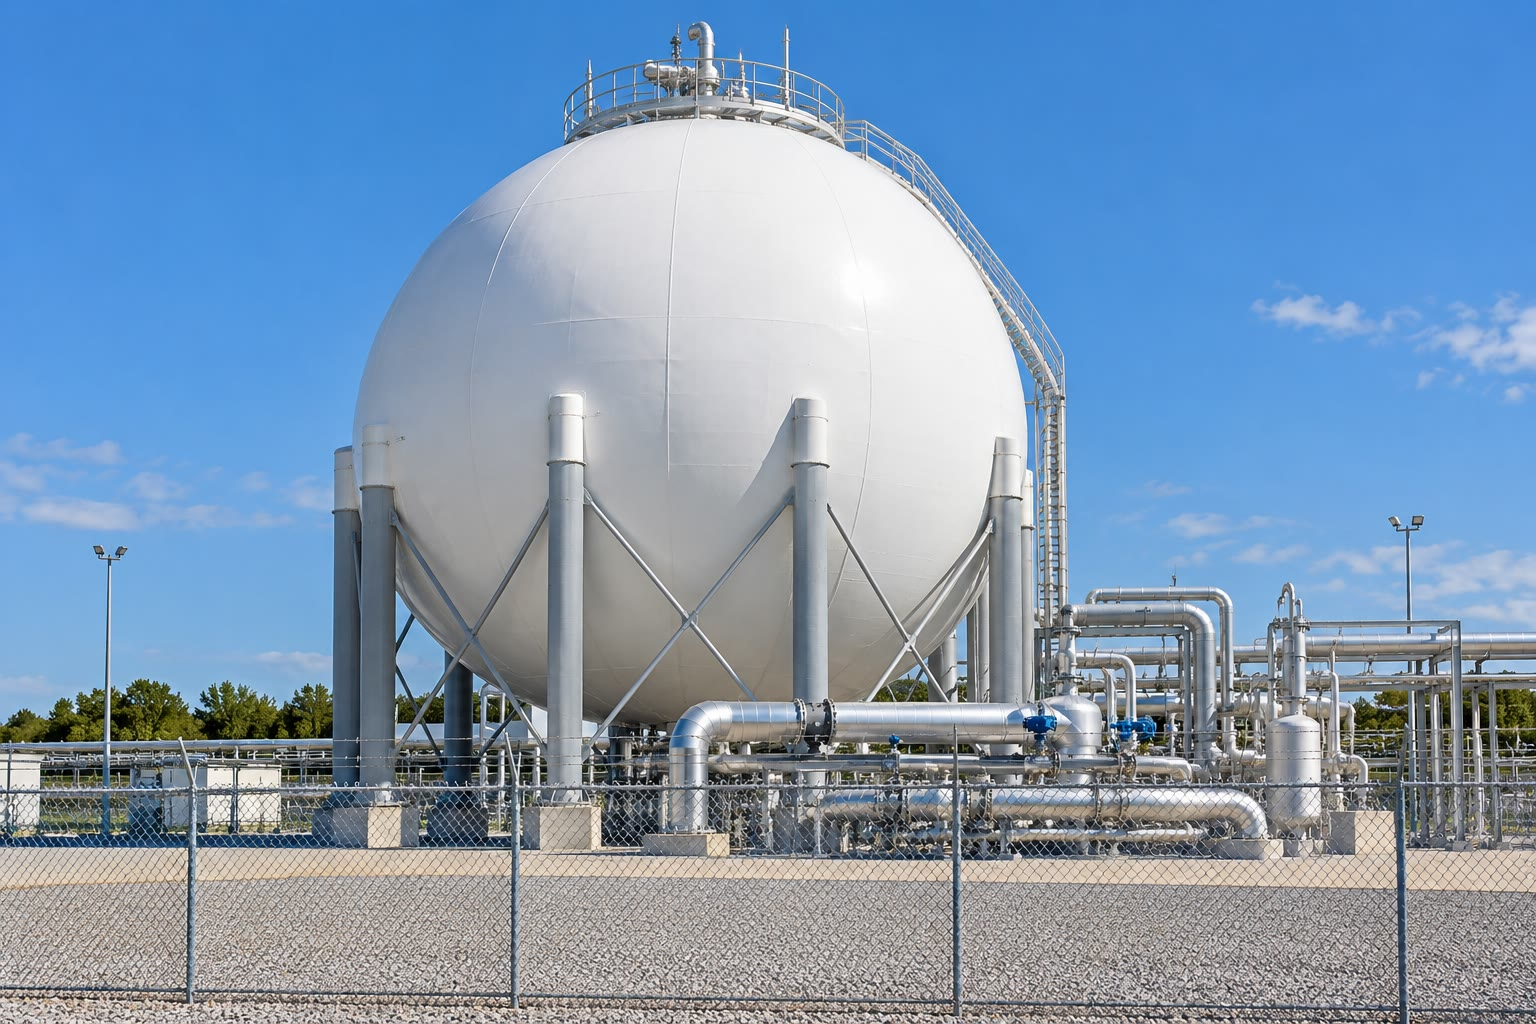
\includegraphics[width=0.6\linewidth]{images/book4/ai/b3-11-lh2-tank.jpg}

{\small Un réservoir sphérique d'hydrogène liquide. À \qty{20}{K}, la
chaleur produite à l'intérieur du liquide par la lente conversion d'une
forme de spin nucléaire du dihydrogène en l'autre peut dépasser la
chaleur qui pénètre de l'extérieur.}
\end{omfigure}

\section{Capacités thermiques des gaz}

La capacité thermique à volume constant vaut $C_V = (\partial U/\partial T)_V$, et
d'après le \cref{thm:b3:partition-functions:internal-energy}, chaque type
de mouvement contribue séparément. Deux limites gouvernent tout.

\begin{theorem}[Théorème d'équipartition]\label{thm:b3:statistical-thermo-applied:equipartition}
Quand les niveaux d'énergie d'un mouvement sont très rapprochés par
rapport à $kT$, chaque terme de son énergie quadratique en une
coordonnée ou en une quantité de mouvement contribue pour
$\frac12kT$ à l'énergie moyenne d'une molécule, donc pour $\frac12R$ à
la capacité thermique molaire. Cet énoncé est le \emph{théorème
d'équipartition}\index{theoreme d'equipartition@théorème d'équipartition}.
\end{theorem}

\begin{proof}[Démonstration partielle]
Dans la limite classique, la somme sur les états d'un mouvement devient
une intégrale, et un terme quadratique $a u^2$ apporte le facteur
$\int\eu^{-\beta au^2}\dd u =
\sqrt{\pi/\beta a}$, proportionnel à $\beta^{-1/2}$. D'après le
\cref{thm:b3:partition-functions:internal-energy}, son énergie moyenne
vaut $-\partial\ln(\beta^{-1/2})/\partial\beta = 1/2\beta = \frac12kT$. Que
l'intégrale classique soit la limite de la somme quantique a été montré
pour la translation et la rotation au
\cref{ch:b3:partition-functions}~; pour la vibration, cela découle de la
proposition suivante quand $T \gg \theta_{\mathrm V}$.
\end{proof}

La translation a trois termes quadratiques ($\frac32R$)~; la rotation
d'une molécule linéaire en a deux ($R$), celle d'une molécule non
linéaire trois ($\frac32R$)~; chaque vibration deux, cinétique et
potentiel ($R$). Une molécule linéaire de $N$ atomes tend donc vers
$C_{V,\mathrm m} = \frac52R + (3N - 5)R$ à haute température. Pour les
vibrations, la limite n'est presque jamais atteinte à température
ambiante.

\begin{proposition}[Capacité thermique de vibration]\label{prop:b3:statistical-thermo-applied:cv-vib}
Une vibration harmonique de température caractéristique
$\theta_{\mathrm V}$ apporte, avec
$x = \theta_{\mathrm V}/T$,
\[
  \frac{C_{V,\mathrm m}^{\mathrm V}}{R} = \frac{x^2\eu^x}{(\eu^x - 1)^2},
\]
la fonction d'Einstein, qui tend vers 1 quand $T \gg \theta_{\mathrm V}$
et décroît exponentiellement, comme $x^2\eu^{-x}$, quand
$T \ll \theta_{\mathrm V}$.
\end{proposition}

\begin{proof}
D'après la \cref{prop:b3:partition-functions:q-vib}, $U - U(0) = R\theta_{\mathrm V}/(\eu^x - 1)$
par mole. En dérivant par rapport à $T$, avec $\dd x/\dd T = -x/T$, on
obtient
$R\theta_{\mathrm V}\eu^x(x/T)/(\eu^x - 1)^2 = Rx^2\eu^x/(\eu^x - 1)^2$. Pour $x \to 0$, $\eu^x - 1 \approx x$ et le
rapport tend vers 1~; pour $x$ grand, il se comporte comme $x^2\eu^{-x}$.
\end{proof}

\begin{method}[La capacité thermique d'un gaz à partir de ses modes]\label{met:b3:statistical-thermo-applied:cv}
\begin{enumerate}
  \item Translation~: $\frac32R$, toujours.
  \item Rotation~: $R$ (molécule linéaire) ou $\frac32R$ (non linéaire)
        si $T \gg \theta_{\mathrm R}$, ce qui est vrai pour tout
        gaz autre que l'hydrogène au-delà de quelques dizaines de kelvins.
  \item Vibrations~: un terme d'Einstein par \omterm{def:b3:group-theory-applied:normal-mode}{mode normal}, avec
        $\theta_{\mathrm V} = hc\tilde\nu/k$ tiré
        des nombres d'onde fondamentaux~; un mode dégénéré compte autant
        de fois que sa \omterm{def:b3:quantum-model-systems:degenerate}{dégénérescence}.
  \item Additionner~; et $C_{p,\mathrm m} = C_{V,\mathrm m} + R$ pour un
        gaz parfait.
\end{enumerate}
\end{method}

Un mouvement est dit gelé quand $kT$ est petit devant sa première
excitation~: il ne stocke alors aucune énergie et ne contribue en rien à
$C_V$. La vibration de \ce{N2} ($\theta_{\mathrm V} = \qty{3352}{K}$) est
gelée à température ambiante et
$C_{V,\mathrm m} = \frac52R$~; celle de \ce{Cl2}
($\theta_{\mathrm V} = \qty{798}{K}$) est à demi éveillée,
$C_{V,\mathrm m} = 3.07R$ à \qty{300}{K}.

\begin{omfigure}
\begin{tikzpicture}
\begin{axis}[width=0.86\linewidth, height=6.4cm, xmode=log, xmin=10, xmax=3000,
  ymin=1.3, ymax=3.9, axis lines=left, xlabel={$T$ / K}, ylabel={$C_{V,\mathrm m}/R$},
  tick label style={font=\small}, label style={font=\small},
  log ticks with fixed point, xtick={10,30,100,300,1000,3000},
  unbounded coords=jump]
\addplot[omDef, thick] table[x=T, y=N2] {figdata/out/bachelor-3-heat-capacity.dat};
\addplot[black!60, thick] table[x=T, y=Cl2] {figdata/out/bachelor-3-heat-capacity.dat};
\addplot[omThm, thick, dashed] table[x=T, y=nH2] {figdata/out/bachelor-3-heat-capacity.dat};
\addplot[omThm, thick] table[x=T, y=eH2] {figdata/out/bachelor-3-heat-capacity.dat};
\addplot[only marks, mark=*, mark size=1.6pt, omDef] table[x=T, y=N2] {figdata/out/bachelor-3-heat-capacity-janaf.dat};
\addplot[only marks, mark=square*, mark size=1.5pt, black!60] table[x=T, y=Cl2] {figdata/out/bachelor-3-heat-capacity-janaf.dat};
\draw[black!30, densely dotted] (axis cs:10,1.5) -- (axis cs:3000,1.5);
\draw[black!30, densely dotted] (axis cs:10,2.5) -- (axis cs:3000,2.5);
\draw[black!30, densely dotted] (axis cs:10,3.5) -- (axis cs:3000,3.5);
\node[font=\scriptsize, black!60, anchor=south east] at (axis cs:2900,1.5) {$\frac32$~: translation};
\node[font=\scriptsize, black!60, anchor=south west] at (axis cs:10.5,2.5) {$\frac52$~: + rotation};
\node[font=\scriptsize, black!60, anchor=south west] at (axis cs:10.5,3.5) {$\frac72$~: + vibration};
\node[font=\scriptsize, omThm, anchor=south west] at (axis cs:60,3.6) {\ce{H2} à l'équilibre};
\node[font=\scriptsize, omThm, anchor=north west] at (axis cs:130,1.78) {\ce{H2} normal};
\node[font=\scriptsize, black!70, anchor=south east] at (axis cs:560,3.33) {\ce{Cl2}};
\node[font=\scriptsize, omDef, anchor=south east] at (axis cs:1000,3.0) {\ce{N2}};
\end{axis}
\end{tikzpicture}

{\small Capacité thermique molaire à volume constant, calculée à partir
des constantes spectroscopiques (traits~; \omterm{def:b3:quantum-model-systems:rotor}{rotateur rigide}, vibration
harmonique), avec les valeurs des tables thermochimiques pour \ce{N2} et
\ce{Cl2} (points, $C_p/R - 1$). La vibration s'éveille vers
$\theta_{\mathrm V}/10$~; au-delà d'environ \qty{1000}{K}, les tables
passent au-dessus du modèle harmonique, qui ignore l'anharmonicité.
Hydrogène~: la contribution de rotation de l'hydrogène normal (en
tirets, ortho et para gelés dans le rapport 3:1) et de l'hydrogène à
l'équilibre (trait plein), qui dépasse $\frac52$ parce que la conversion
du para en ortho absorbe de la chaleur.}
\end{omfigure}

\section{Statistique de spin nucléaire}

Les deux noyaux de \ce{H2} sont des fermions identiques. Les échanger
change le signe de la fonction d'onde totale
(\cref{ch:b3:many-electron-atoms})~; les échanger revient à retourner la
molécule bout pour bout, ce qui multiplie la fonction d'onde de rotation
$Y_{J,M}$ par $(-1)^J$ et la fonction de spin nucléaire par $+1$ ou par
$-1$.

\begin{theorem}[Statistique de spin nucléaire]\label{thm:b3:statistical-thermo-applied:spin-statistics}
Dans une molécule diatomique homonucléaire dont les noyaux ont le spin
$I$, dans un état électronique fondamental ${}^1\Sigma_g^+$, il existe
$(2I+1)(I+1)$ états de spin nucléaire symétriques et $(2I+1)I$
antisymétriques. Pour des fermions ($I$ demi-entier), les états
antisymétriques vont avec les $J$ pairs et les symétriques avec les $J$
impairs~; pour des bosons ($I$ entier), c'est l'inverse. Pour \ce{H2}
($I = \frac12$), les niveaux pairs et impairs ont les poids de spin 1 et
3~; pour \ce{D2} ($I = 1$), 6 et 3. Quand $I = 0$, une seule parité de
$J$ existe~: la molécule linéaire \ce{CO2}, avec deux noyaux \ce{^{16}O}
et un état fondamental symétrique, n'a que des niveaux de rotation pairs.
\end{theorem}

\begin{proof}[Démonstration partielle]
Le postulat de symétrisation (la fonction d'onde totale est
antisymétrique par échange de deux fermions identiques, symétrique pour
des bosons) est admis. Les
$(2I+1)^2$ produits d'états de spin d'un noyau $|m_1\rangle|m_2\rangle$
donnent $2I+1$ états symétriques
avec $m_1 = m_2$, et pour chacune des $(2I+1)2I/2$ paires $m_1 \ne m_2$
une combinaison symétrique et une antisymétrique~: $(2I+1) + (2I+1)I = (2I+1)(I+1)$
états symétriques et $(2I+1)I$ antisymétriques. Dans un état
${}^1\Sigma_g^+$, les fonctions électronique et de vibration sont
inchangées par l'échange, si bien que le produit des fonctions de
rotation et de spin doit avoir le signe global requis~: pour des
fermions, $(-1)^J \times(\text{symétrie de spin}) = -1$, ce qui associe
les $J$ pairs aux états de spin antisymétriques. Pour \ce{H2}~: 3
symétriques, 1 antisymétrique~; pour \ce{D2}~: 6 et
3.
\end{proof}

\begin{definition}[Orthohydrogène et parahydrogène]\label{def:b3:statistical-thermo-applied:spin-isomers}
L'\emph{orthohydrogène}\index{orthohydrogene@orthohydrogène} est la forme
de \ce{H2} dont les deux spins des protons sont dans un état symétrique
(triplet), qui n'occupe que les niveaux de rotation impairs~; le
\emph{parahydrogène}\index{parahydrogene@parahydrogène} est la forme dont
l'état de spin est antisymétrique (singulet), qui n'occupe que les
niveaux pairs.
\end{definition}

Convertir l'une en l'autre exige de retourner un spin nucléaire par
rapport à l'autre, ce que les collisions avec d'autres molécules de
dihydrogène ne font presque pas~: dans l'hydrogène pur, les deux formes
se comportent pendant des jours comme deux gaz différents. Une surface
paramagnétique, dont le champ magnétique inhomogène agit différemment sur
les deux protons, catalyse la conversion.

\begin{proposition}[Rapport ortho--para à l'équilibre]\label{prop:b3:statistical-thermo-applied:ortho-para}
À l'équilibre, la fraction de \omterm{def:b3:statistical-thermo-applied:spin-isomers}{parahydrogène} vaut
\[
  x_{\mathrm{para}} = \frac{\sum_{J\,\mathrm{even}}(2J+1)\eu^{-\theta_{\mathrm R}J(J+1)/T}}
    {\sum_{J\,\mathrm{even}}(2J+1)\eu^{-\theta_{\mathrm R}J(J+1)/T} + 3\sum_{J\,\mathrm{odd}}(2J+1)\eu^{-\theta_{\mathrm R}J(J+1)/T}},
\]
qui tend vers 1 à 0 K et vers $\frac14$ à haute température. Pour
\ce{D2}, la forme ortho
($J$ pairs) tend vers 1 à 0 K et vers $\frac23$ à haute température.
\end{proposition}

\begin{proof}
C'est la \omterm{def:b3:partition-functions:boltzmann}{distribution de Boltzmann} sur tous les états, avec les poids de
spin du
\cref{thm:b3:statistical-thermo-applied:spin-statistics}. À 0 K, seul
$J = 0$, qui est pair, est peuplé. À haute température, les sommes paire
et impaire valent chacune la moitié
de $T/\theta_{\mathrm R}$, et le rapport vaut $1 : 3$~; pour \ce{D2}, $6 : 3$.
\end{proof}

Pour \ce{H2}, $\theta_{\mathrm R} = \qty{85.4}{K}$~: le mélange à
l'équilibre contient moitié de para à \qty{78}{K},
99.8\,\% de para au point d'ébullition, \qty{20.37}{K}, et 25.07\,\% à
température ambiante. L'hydrogène conservé à température ambiante,
appelé hydrogène normal, est donc un mélange 3:1 d'ortho et de para.

\begin{omfigure}
\begin{tikzpicture}
\begin{axis}[width=0.72\linewidth, height=5.4cm, xmin=0, xmax=300, ymin=0, ymax=1.05,
  axis lines=left, xlabel={$T$ / K}, ylabel={fraction à l'équilibre},
  tick label style={font=\small}, label style={font=\small}]
\addplot[omThm, thick] table[x=T, y=pH2] {figdata/out/bachelor-3-ortho-para.dat};
\addplot[omDef, thick] table[x=T, y=oD2] {figdata/out/bachelor-3-ortho-para.dat};
\draw[black!35, densely dotted] (axis cs:0,0.25) -- (axis cs:300,0.25);
\draw[black!35, densely dotted] (axis cs:0,0.6667) -- (axis cs:300,0.6667);
\node[font=\scriptsize, omThm, anchor=south west] at (axis cs:190,0.27) {fraction para de \ce{H2} $\to \frac14$};
\node[font=\scriptsize, omDef, anchor=south west] at (axis cs:120,0.69) {fraction ortho de \ce{D2} $\to \frac23$};
\end{axis}
\end{tikzpicture}

{\small Composition à l'équilibre des isomères de spin nucléaire en
fonction de la température, à partir des niveaux de rotation et des
poids de spin (\ce{H2}~: 1 et 3~;
\ce{D2}~: 6 et 3). Les deux formes de $J$ pair l'emportent à basse
température.}
\end{omfigure}

La capacité thermique de l'hydrogène en montre les conséquences. Dans
l'hydrogène normal, les molécules ortho et para sont deux gaz mélangés
en proportions fixes~; chacun a sa propre échelle de niveaux, commençant
à $J = 1$ et à $J = 0$, et sa rotation se gèle séparément. Dans
l'hydrogène à l'équilibre, le chauffage convertit aussi du para en
ortho, ce qui absorbe de l'énergie et donne le pic de la figure
ci-dessus. Les premières mesures, faites sans catalyseur, suivaient la
courbe de l'hydrogène normal, et c'est l'interprétation de cette courbe
comme celle d'un mélange 3:1 gelé qui a d'abord révélé les deux formes.

\begin{remark}
Le \omterm{def:b3:partition-functions:symmetry-number}{nombre de symétrie} de la \cref{prop:b3:partition-functions:q-rot} est
maintenant justifié.
À haute température, chaque état de spin trouve environ la moitié des
niveaux de rotation permis, de sorte que
$\sum(\text{poids de spin})(2J+1)\eu^{\dots} \approx (2I+1)^2\,T/2\theta_{\mathrm R}$~:
le facteur de spin total $(2I+1)^2$ est omis par convention, et il reste
$\sigma = 2$.
\end{remark}

\begin{definition}[Entropie résiduelle]\label{def:b3:statistical-thermo-applied:residual-entropy}
L'\emph{entropie résiduelle}\index{entropie residuelle@entropie résiduelle} d'un cristal est l'entropie
qu'il conserve quand $T \to 0$ parce que ses molécules restent figées
dans l'un de nombreux arrangements d'énergies égales ou presque égales.
\end{definition}

\begin{proposition}[Entropies résiduelles du monoxyde de carbone et de la glace]\label{prop:b3:statistical-thermo-applied:residual}
Un cristal de $N$ molécules figé dans $W_0$ arrangements équiprobables a
$S_0 =
k\ln W_0$. Le \ce{CO} solide, chaque molécule pointant dans un sens ou
dans l'autre, a $S_{0,\mathrm m} = R\ln2 =
\qty{5.76}{J.K^{-1}.mol^{-1}}$. La glace, où chaque oxygène est lié à
deux atomes d'hydrogène et lié par liaison hydrogène à deux autres, a
$W_0 = (3/2)^N$ et $S_{0,\mathrm m} = R\ln\frac32 =
\qty{3.37}{J.K^{-1}.mol^{-1}}$.
\end{proposition}

\begin{proof}
Application de la \cref{def:b3:partition-functions:statistical-entropy}
pour $T \to 0$.
\ce{CO}~: le dipôle de la molécule est si petit que les orientations CO
et OC ont presque la même énergie, et chacune des $N$ molécules en a
deux~: $W_0 = 2^N$,
$S_0 = Nk\ln2$. Glace (dénombrement de Pauling)~: chacun des $2N$ atomes
d'hydrogène se trouve sur une droite
O$\cdots$O, près de l'une ou de l'autre extrémité~: $2^{2N}$
arrangements. Des 16 façons de placer les quatre hydrogènes autour d'un
oxygène, 6 lui donnent exactement deux hydrogènes proches (une molécule
d'eau)~; en traitant les oxygènes comme indépendants, une fraction
$6/16$ des arrangements satisfait chacun d'eux~: $W_0 = 2^{2N}(6/16)^N = (3/2)^N$.
\end{proof}

Pour \ce{CO}, les tables donnent l'\omterm{def:b3:partition-functions:statistical-entropy}{entropie statistique}
(\cref{ch:b3:partition-functions})~; la valeur calorimétrique est plus
basse d'un écart de l'ordre de $R\ln2$, un peu moindre parce que les
orientations ne sont pas tout à fait aléatoires. Pour la glace, l'écart
entre l'entropie calorimétrique de la vapeur d'eau et sa valeur
statistique concordait avec le dénombrement de Pauling quand celui-ci le
fit en 1935, confirmant que les protons de la glace sont désordonnés. Le
troisième principe, sous la forme «~l'entropie d'un cristal parfait est
nulle à 0 K~», s'applique aux cristaux qui atteignent effectivement un
arrangement unique.

\begin{omfigure}
\begin{tikzpicture}[scale=1.15, every node/.style={transform shape}]
  \draw[black!45, dashed] (0.00,0.00) -- (1.20,0.00);
  \draw[black, thick] (0.00,0.00) -- (0.36,0.00); \node[aH, minimum size=2.2mm] at (0.36,0.00) {};
  \draw[black!45, dashed] (0.00,0.00) -- (0.00,1.20);
  \draw[black, thick] (0.00,0.00) -- (0.00,0.36); \node[aH, minimum size=2.2mm] at (0.00,0.36) {};
  \draw[black!45, dashed] (0.00,1.20) -- (1.20,1.20);
  \draw[black, thick] (0.00,1.20) -- (0.36,1.20); \node[aH, minimum size=2.2mm] at (0.36,1.20) {};
  \draw[black!45, dashed] (0.00,1.20) -- (0.00,2.40);
  \draw[black, thick] (0.00,2.40) -- (0.00,2.04); \node[aH, minimum size=2.2mm] at (0.00,2.04) {};
  \draw[black!45, dashed] (0.00,2.40) -- (1.20,2.40);
  \draw[black, thick] (1.20,2.40) -- (0.84,2.40); \node[aH, minimum size=2.2mm] at (0.84,2.40) {};
  \draw[black!45, dashed] (0.00,2.40) -- (0.00,3.60);
  \draw[black, thick] (0.00,3.60) -- (0.00,3.24); \node[aH, minimum size=2.2mm] at (0.00,3.24) {};
  \draw[black!45, dashed] (0.00,3.60) -- (1.20,3.60);
  \draw[black, thick] (1.20,3.60) -- (0.84,3.60); \node[aH, minimum size=2.2mm] at (0.84,3.60) {};
  \draw[black!45, dashed] (0.00,3.60) -- (0.00,4.20);
  \draw[black, thick] (0.00,3.60) -- (0.00,3.96); \node[aH, minimum size=2.2mm] at (0.00,3.96) {};
  \draw[black!45, dashed] (1.20,0.00) -- (2.40,0.00);
  \draw[black, thick] (1.20,0.00) -- (1.56,0.00); \node[aH, minimum size=2.2mm] at (1.56,0.00) {};
  \draw[black!45, dashed] (1.20,0.00) -- (1.20,1.20);
  \draw[black, thick] (1.20,1.20) -- (1.20,0.84); \node[aH, minimum size=2.2mm] at (1.20,0.84) {};
  \draw[black!45, dashed] (1.20,1.20) -- (2.40,1.20);
  \draw[black, thick] (2.40,1.20) -- (2.04,1.20); \node[aH, minimum size=2.2mm] at (2.04,1.20) {};
  \draw[black!45, dashed] (1.20,1.20) -- (1.20,2.40);
  \draw[black, thick] (1.20,1.20) -- (1.20,1.56); \node[aH, minimum size=2.2mm] at (1.20,1.56) {};
  \draw[black!45, dashed] (1.20,2.40) -- (2.40,2.40);
  \draw[black, thick] (1.20,2.40) -- (1.56,2.40); \node[aH, minimum size=2.2mm] at (1.56,2.40) {};
  \draw[black!45, dashed] (1.20,2.40) -- (1.20,3.60);
  \draw[black, thick] (1.20,3.60) -- (1.20,3.24); \node[aH, minimum size=2.2mm] at (1.20,3.24) {};
  \draw[black!45, dashed] (1.20,3.60) -- (2.40,3.60);
  \draw[black, thick] (2.40,3.60) -- (2.04,3.60); \node[aH, minimum size=2.2mm] at (2.04,3.60) {};
  \draw[black!45, dashed] (1.20,3.60) -- (1.20,4.20);
  \draw[black!45, dashed] (2.40,0.00) -- (3.60,0.00);
  \draw[black, thick] (3.60,0.00) -- (3.24,0.00); \node[aH, minimum size=2.2mm] at (3.24,0.00) {};
  \draw[black!45, dashed] (2.40,0.00) -- (2.40,1.20);
  \draw[black, thick] (2.40,0.00) -- (2.40,0.36); \node[aH, minimum size=2.2mm] at (2.40,0.36) {};
  \draw[black!45, dashed] (2.40,1.20) -- (3.60,1.20);
  \draw[black, thick] (2.40,1.20) -- (2.76,1.20); \node[aH, minimum size=2.2mm] at (2.76,1.20) {};
  \draw[black!45, dashed] (2.40,1.20) -- (2.40,2.40);
  \draw[black, thick] (2.40,2.40) -- (2.40,2.04); \node[aH, minimum size=2.2mm] at (2.40,2.04) {};
  \draw[black!45, dashed] (2.40,2.40) -- (3.60,2.40);
  \draw[black, thick] (3.60,2.40) -- (3.24,2.40); \node[aH, minimum size=2.2mm] at (3.24,2.40) {};
  \draw[black!45, dashed] (2.40,2.40) -- (2.40,3.60);
  \draw[black, thick] (2.40,2.40) -- (2.40,2.76); \node[aH, minimum size=2.2mm] at (2.40,2.76) {};
  \draw[black!45, dashed] (2.40,3.60) -- (3.60,3.60);
  \draw[black, thick] (2.40,3.60) -- (2.76,3.60); \node[aH, minimum size=2.2mm] at (2.76,3.60) {};
  \draw[black!45, dashed] (2.40,3.60) -- (2.40,4.20);
  \draw[black!45, dashed] (3.60,0.00) -- (4.20,0.00);
  \draw[black, thick] (3.60,0.00) -- (3.96,0.00); \node[aH, minimum size=2.2mm] at (3.96,0.00) {};
  \draw[black!45, dashed] (3.60,0.00) -- (3.60,1.20);
  \draw[black, thick] (3.60,1.20) -- (3.60,0.84); \node[aH, minimum size=2.2mm] at (3.60,0.84) {};
  \draw[black!45, dashed] (3.60,1.20) -- (4.20,1.20);
  \draw[black!45, dashed] (3.60,1.20) -- (3.60,2.40);
  \draw[black, thick] (3.60,1.20) -- (3.60,1.56); \node[aH, minimum size=2.2mm] at (3.60,1.56) {};
  \draw[black!45, dashed] (3.60,2.40) -- (4.20,2.40);
  \draw[black!45, dashed] (3.60,2.40) -- (3.60,3.60);
  \draw[black, thick] (3.60,2.40) -- (3.60,2.76); \node[aH, minimum size=2.2mm] at (3.60,2.76) {};
  \draw[black!45, dashed] (3.60,3.60) -- (4.20,3.60);
  \draw[black, thick] (3.60,3.60) -- (3.96,3.60); \node[aH, minimum size=2.2mm] at (3.96,3.60) {};
  \draw[black!45, dashed] (3.60,3.60) -- (3.60,4.20);
  \draw[black, thick] (3.60,3.60) -- (3.60,3.96); \node[aH, minimum size=2.2mm] at (3.60,3.96) {};
  \draw[black!45, dashed] (-0.60,0.00) -- (0.00,0.00);
  \draw[black!45, dashed] (-0.60,1.20) -- (0.00,1.20);
  \draw[black, thick] (0.00,1.20) -- (-0.36,1.20); \node[aH, minimum size=2.2mm] at (-0.36,1.20) {};
  \draw[black!45, dashed] (-0.60,2.40) -- (0.00,2.40);
  \draw[black, thick] (0.00,2.40) -- (-0.36,2.40); \node[aH, minimum size=2.2mm] at (-0.36,2.40) {};
  \draw[black!45, dashed] (-0.60,3.60) -- (0.00,3.60);
  \draw[black!45, dashed] (0.00,-0.60) -- (0.00,0.00);
  \draw[black!45, dashed] (1.20,-0.60) -- (1.20,0.00);
  \draw[black, thick] (1.20,0.00) -- (1.20,-0.36); \node[aH, minimum size=2.2mm] at (1.20,-0.36) {};
  \draw[black!45, dashed] (2.40,-0.60) -- (2.40,0.00);
  \draw[black, thick] (2.40,0.00) -- (2.40,-0.36); \node[aH, minimum size=2.2mm] at (2.40,-0.36) {};
  \draw[black!45, dashed] (3.60,-0.60) -- (3.60,0.00);
  \node[aO, minimum size=4mm] at (0.00,0.00) {};
  \node[aO, minimum size=4mm] at (0.00,1.20) {};
  \node[aO, minimum size=4mm] at (0.00,2.40) {};
  \node[aO, minimum size=4mm] at (0.00,3.60) {};
  \node[aO, minimum size=4mm] at (1.20,0.00) {};
  \node[aO, minimum size=4mm] at (1.20,1.20) {};
  \node[aO, minimum size=4mm] at (1.20,2.40) {};
  \node[aO, minimum size=4mm] at (1.20,3.60) {};
  \node[aO, minimum size=4mm] at (2.40,0.00) {};
  \node[aO, minimum size=4mm] at (2.40,1.20) {};
  \node[aO, minimum size=4mm] at (2.40,2.40) {};
  \node[aO, minimum size=4mm] at (2.40,3.60) {};
  \node[aO, minimum size=4mm] at (3.60,0.00) {};
  \node[aO, minimum size=4mm] at (3.60,1.20) {};
  \node[aO, minimum size=4mm] at (3.60,2.40) {};
  \node[aO, minimum size=4mm] at (3.60,3.60) {};
\end{tikzpicture}

{\small Le désordre des protons dans la glace, dessiné comme un réseau
carré plan (le réseau réel est tétraédrique)~: chaque oxygène (rouge) a
quatre voisins O$\cdots$O, un hydrogène (blanc) sur chaque droite, et
exactement deux hydrogènes proches de lui (les règles de la glace).
C'est l'un des $(3/2)^N$ arrangements du dénombrement de Pauling~; tous
ont presque la même énergie, et la congélation en choisit un au hasard.}
\end{omfigure}

\section{Constantes d'équilibre et fonctions de partition}

\begin{theorem}[Constante d'équilibre à partir des fonctions de partition]\label{thm:b3:statistical-thermo-applied:k-from-q}
Pour une réaction $0 = \sum_J\nu_J\mathrm J$ entre gaz parfaits,
\[
  K^\circ = \prod_J\Bigl(\frac{q^\circ_{J,\mathrm m}}{N_A}\Bigr)^{\nu_J}\eu^{-\Delta_rE_0/RT},
\]
où $q^\circ_{J,\mathrm m}$ est la fonction de partition de $\mathrm J$
dans le volume molaire standard
$V^\circ_{\mathrm m} = RT/p^\circ$, chacune comptée à partir de son
propre état fondamental, et $\Delta_rE_0 =
\sum\nu_JE_{0,J}$ est l'énergie molaire de réaction à 0 K, de l'état
fondamental des réactifs à celui des produits.
\end{theorem}

\begin{proof}
D'après le \cref{thm:b3:partition-functions:entropy}, une mole de gaz
parfait $\mathrm J$ sous $p^\circ$ a
$G^\circ_{\mathrm m} - G_{\mathrm m}(0) = -RT\ln(q^\circ_{J,\mathrm m}/N_A)$, et $G_{\mathrm m}(0)$ est l'énergie $E_{0,J}$
de son état fondamental sur une échelle commune à toutes les espèces.
Donc $\Delta_rG^\circ =
\Delta_rE_0 - RT\sum_J\nu_J\ln(q^\circ_{J,\mathrm m}/N_A)$, et $\Delta_rG^\circ = -RT\ln K^\circ$
donne le résultat.
\end{proof}

\begin{method}[Calculer une constante d'équilibre à partir de données spectroscopiques]\label{met:b3:statistical-thermo-applied:k-stat}
\begin{enumerate}
  \item Pour chaque espèce~: $q^\circ_{\mathrm m}/N_A = (kT/p^\circ)\Lambda^{-3}\times q^{\mathrm R}q^{\mathrm V}q^{\mathrm E}$,
        avec les \omterm{def:b3:partition-functions:symmetry-number}{nombres de symétrie} et les \omterm{def:b3:quantum-model-systems:degenerate}{dégénérescences}
        électroniques.
  \item $\Delta_rE_0$ à partir des énergies de dissociation $D_0$
        (mesurées depuis le niveau de vibration fondamental, si bien que
        les \omterm{def:b3:quantum-model-systems:oscillator}{énergies de point zéro} sont incluses) ou des enthalpies de
        formation à 0 K.
  \item Multiplier, et vérifier les unités~: $K^\circ$ est un nombre pur,
        la pression standard intervenant par $kT/p^\circ$.
\end{enumerate}
\end{method}

\begin{example}[La dissociation du diiode]\label{ex:b3:statistical-thermo-applied:iodine}
% ledger: janaf:I.dfH0, janaf:I2g.dfH0, lev:I.2P1_2, diat:I2.we, diat:I2.wexe, diat:I2.Be, diat:I2.ae, aw:I, janaf:I.logKf.1000
Pour $\ce{I2(g) <=> 2 I(g)}$, $\Delta_rE_0 = D_0(\ce{I2}) = 2 \times 107.164 - 65.504 = \qty{148.824}{kJ/mol}$
d'après les enthalpies de formation à 0 K des tables thermochimiques. À
\qty{1000}{K}~: pour I, $\Lambda = \qty{4.90}{pm}$, $kT/p^\circ = \qty{1.381e-25}{m^3}$, $q^{\mathrm E} = 4 +
2\eu^{-10.94} = 4.0000$ (le niveau ${}^2P_{1/2}$ se situe \qty{7603}{cm^{-1}}
plus haut), donc $q^\circ_{\mathrm m}/N_A = \num{4.69e9}$~;
pour \ce{I2}, $\Lambda = \qty{3.47}{pm}$, $q^{\mathrm R} = 1000/(2 \times 0.05369) = 9313$ et $q^{\mathrm V} = 3.784$, donc
$q^\circ_{\mathrm m}/N_A = \num{1.17e14}$. Alors $K^\circ = (4.69\times10^9)^2/(1.17\times10^{14}) \times \eu^{-17.90} =
\num{3.17e-3}$, $\log K^\circ = -2.50$~; les tables donnent $-2.51$.
\end{example}

\begin{omfigure}
\begin{tikzpicture}
\begin{axis}[name=ki, width=0.5\linewidth, height=5.6cm, xmin=0.58, xmax=1.45, ymin=-6.5,
  ymax=1, axis lines=left, xlabel={$1000\,\mathrm K/T$}, ylabel={$\log K^\circ$},
  tick label style={font=\small}, label style={font=\small},
  title={\small $\ce{I2 <=> 2 I}$}]
\addplot[black, thick] table[x=invT, y=logK] {figdata/out/bachelor-3-equilibrium-constant-stat-i2.dat};
\addplot[only marks, mark=*, mark size=1.8pt, omThm] table[x=invT, y=logK] {figdata/out/bachelor-3-equilibrium-constant-stat-i2-janaf.dat};
\node[font=\scriptsize, anchor=north east, align=right] at (axis cs:1.43,0.8) {trait~: statistique\\ points~: tables};
\end{axis}
\begin{axis}[at={(ki.east)}, anchor=west, xshift=1.4cm, width=0.44\linewidth, height=5.6cm,
  xmin=0, xmax=2000, ymin=0, ymax=4.4, axis lines=left, xlabel={$T$ / K},
  ylabel={$K^\circ$}, tick label style={font=\small}, label style={font=\small},
  title={\small $\ce{H2 + D2 <=> 2 HD}$}, scaled x ticks=false,
  xticklabel style={/pgf/number format/1000 sep={}}]
\addplot[omDef, thick] table[x=T, y=K] {figdata/out/bachelor-3-equilibrium-constant-stat-hd.dat};
\draw[black!35, densely dotted] (axis cs:0,4) -- (axis cs:2000,4);
\node[font=\scriptsize, anchor=north east] at (axis cs:1950,3.95) {limite de $\sigma$~: 4};
\end{axis}
\end{tikzpicture}

{\small Constantes d'équilibre calculées à partir des fonctions de
partition. À gauche~: la dissociation du diiode, une droite de van 't
Hoff de pente $-\Delta_rH^\circ/(R\ln10)$, avec
les valeurs des tables thermochimiques (points). À droite~: l'échange $\ce{H2 + D2
<=> 2 HD}$, qui tend vers le rapport des \omterm{def:b3:partition-functions:symmetry-number}{nombres de symétrie}, 4, à haute
température et passe au-dessous à basse température à cause des
\omterm{def:b3:quantum-model-systems:oscillator}{énergies de point zéro} et des restrictions de spin nucléaire.}
\end{omfigure}

\begin{proposition}[L'échange H$_2$ + D$_2$]\label{prop:b3:statistical-thermo-applied:hd}
Pour $\ce{H2 + D2 <=> 2 HD}$, $K^\circ \to 4$ à haute température.
\end{proposition}

\begin{proof}
À haute température, les facteurs de translation, de rotation et de
vibration valent
$m^{3/2}$, $T/\sigma\theta_{\mathrm R} \propto \mu/\sigma$ et $T/\theta_{\mathrm V} \propto \sqrt\mu$ (la
\omterm{def:b3:quantum-model-systems:oscillator}{constante de force}, propriété électronique, est la même pour les trois
molécules), et $\Delta_rE_0/RT \to 0$.
Avec $m_{\ce{H2}} = 2$, $m_{\ce{D2}} = 4$, $m_{\ce{HD}} = 3$ et
$\mu = 1/2$, 1, $2/3$ (en unités de la masse du proton, en négligeant la
petite différence entre D et 2H)~:
\[
  K^\circ \to \Bigl(\frac{9}{8}\Bigr)^{3/2} \times \frac{(2/3)^2/1^2}{(1/2)(1)/(2 \times 2)}
  \times \frac{2/3}{\sqrt{1/2}\sqrt1}
  = \frac{27}{16\sqrt2} \times \frac{32}{9} \times \frac{2\sqrt2}{3} = 4 .
\]
Tous les facteurs de masse se simplifient exactement~: seuls restent les
\omterm{def:b3:partition-functions:symmetry-number}{nombres de symétrie}, $\sigma_{\ce{H2}}
\sigma_{\ce{D2}}/\sigma_{\ce{HD}}^2 = 4$.
\end{proof}

À \qty{298.15}{K}, la constante statistique vaut 3.26~: les \omterm{def:b3:quantum-model-systems:oscillator}{énergies de
point zéro} de \ce{H2},
\ce{D2} et HD (\qty{2170.3}{cm^{-1}}, \qty{1542.3}{cm^{-1}} et \qty{1883.7}{cm^{-1}}) donnent $\Delta_rE_0 =
\qty{54.8}{cm^{-1}}$, soit un facteur $\eu^{-54.8/207.2} = 0.77$~; la
rotation, encore en partie quantifiée pour ces molécules légères, compte
aussi.

\begin{proposition}[La relation de van 't Hoff retrouvée]\label{prop:b3:statistical-thermo-applied:vant-hoff-stat}
La constante d'équilibre statistique obéit à $\dfrac{\dd\ln K^\circ}{\dd T} = \dfrac{\Delta_rH^\circ}{RT^2}$.
\end{proposition}

\begin{proof}
Chaque $q^\circ_{J,\mathrm m}$ dépend de $T$ par ses niveaux et par
$V^\circ_{\mathrm m} = RT/p^\circ$~:
$\dd\ln q^\circ_{J,\mathrm m}/\dd T = (U_J - U_J(0))/RT^2 + 1/T$ par
mole, d'après le
\cref{thm:b3:partition-functions:internal-energy}. Donc $\dd\ln K^\circ/\dd T =
[\Delta_rE_0 + \sum\nu_J(U_J - U_J(0)) + \sum\nu_JRT]/RT^2 = (\Delta_rU + \Delta\nu_{\mathrm g}RT)/RT^2 =
\Delta_rH^\circ/RT^2$ pour des gaz parfaits.
\end{proof}

D'après la pente du panneau de gauche de la figure, l'enthalpie de
dissociation du diiode vers \qty{1000}{K} vaut \qty{154}{kJ/mol}~:
$D_0$ plus l'énergie de translation supplémentaire de deux atomes par
rapport à une molécule, moins l'énergie de rotation et de vibration de
celle-ci.

\section{Effets isotopiques}

Les \omterm{def:b3:rovibrational-spectroscopy:rotational-constant}{isotopologues} ont la même structure électronique, donc la même courbe
d'énergie potentielle et les mêmes \omterm{def:b3:quantum-model-systems:oscillator}{constantes de force}, mais des masses
différentes~: leurs nombres d'onde de vibration, leurs \omterm{def:b3:quantum-model-systems:oscillator}{énergies de point
zéro} et leurs fonctions de partition diffèrent, et leurs constantes
d'équilibre aussi.

\begin{definition}[Effet isotopique d'équilibre, facteur de fractionnement, valeur $\delta$]\label{def:b3:statistical-thermo-applied:isotope-effect}
L'\emph{effet isotopique d'équilibre}\index{effet isotopique d'equilibre@effet isotopique d'équilibre} d'une
réaction est le rapport $K_{\mathrm{light}}/K_{\mathrm{heavy}}$ de ses
constantes d'équilibre avec l'isotope léger et avec l'isotope lourd. Le
\emph{facteur de fractionnement}\index{facteur de fractionnement}
entre deux phases ou deux composés A et B est $\alpha_{\mathrm{A/B}} = R_{\mathrm A}/R_{\mathrm B}$, où
$R$ est le rapport de l'isotope lourd à l'isotope léger (par exemple
$\ce{^{18}O}/\ce{^{16}O}$). La
\emph{valeur $\delta$}\index{valeur delta@valeur $\delta$} d'un échantillon est $\delta = (R_{\mathrm{sample}}/R_{\mathrm{standard}}
- 1) \times 1000$, exprimée en pour mille (\textperthousand).
\end{definition}

\begin{proposition}[Effets isotopiques et énergies de point zéro]\label{prop:b3:statistical-thermo-applied:zpe-isotope}
Pour un échange $\ce{XH + YD <=> XD + YH}$, à des températures où les
vibrations d'élongation sont gelées, le facteur dominant de la constante
d'équilibre est
\[
  K \approx \exp\Bigl(-\frac{\Delta\mathrm{ZPE}}{kT}\Bigr), \qquad
  \Delta\mathrm{ZPE} = \tfrac12hc\bigl[\tilde\nu_{\mathrm{XD}} + \tilde\nu_{\mathrm{YH}} - \tilde\nu_{\mathrm{XH}} - \tilde\nu_{\mathrm{YD}}\bigr],
\]
et $\tilde\nu_{\mathrm D} \approx \tilde\nu_{\mathrm H}/\sqrt2$ pour un
hydrogène lié à un atome lourd. L'isotope lourd se concentre dans la
liaison la plus raide.
\end{proposition}

\begin{proof}
Le \Cref{thm:b3:statistical-thermo-applied:k-from-q}, avec les énergies
comptées à partir du fond des courbes de potentiel communes~:
$\Delta_rE_0$ est la variation de l'\omterm{def:b3:quantum-model-systems:oscillator}{énergie de point zéro}. Les facteurs
de translation et de rotation se compensent presque entre deux échanges
des mêmes isotopes sur des partenaires lourds, et les fonctions de
partition de vibration valent 1 quand elles sont gelées. Avec
$\tilde\nu \propto \mu^{-1/2}$ et
$\mu_{\mathrm{XD}} \approx 2\mu_{\mathrm{XH}}$ pour X lourd, $\tilde\nu_{\mathrm{XD}} = \tilde\nu_{\mathrm{XH}}/\sqrt2$, et $\Delta\mathrm{ZPE} =
\frac12hc(1 - 1/\sqrt2)(\tilde\nu_{\mathrm{YH}} - \tilde\nu_{\mathrm{XH}})$~:
négative, donc $K > 1$, quand la liaison X--H est la plus raide.
\end{proof}

Le même raisonnement explique le fractionnement des isotopes de l'oxygène
entre l'eau et sa vapeur, entre l'eau et le carbonate d'une coquille, ou
entre deux minéraux~: le \omterm{def:b3:statistical-thermo-applied:isotope-effect}{facteur de fractionnement} tend vers 1 à haute
température (comme $K_{\mathrm{HD}}$ tend vers sa limite de symétrie) et
s'écarte de 1 quand la température baisse. Mesuré sous forme de valeurs
$\delta$, c'est un thermomètre~: le $\delta^{18}$O du carbonate des
coquilles fossiles enregistre la température de l'eau dans laquelle
elles ont grandi, et celui de la glace des carottes polaires la
température des nuages qui ont formé sa neige.

\begin{inthelab}[Un convertisseur ortho--para]
Un liquéfacteur d'hydrogène refroidit le gaz par étages et, entre les
étages, le fait passer sur des lits d'un catalyseur paramagnétique,
typiquement de l'oxyde de fer(III) hydraté. La chaleur de conversion est
alors évacuée à chaque température par le réfrigérateur, et le liquide
qui arrive dans le réservoir est proche de sa composition d'équilibre,
presque entièrement para. Sans le catalyseur, la chaleur de conversion
serait libérée dans le réservoir.
\end{inthelab}

\begin{safety}{\ghs[0.8cm]{GHS02}\ghs[0.8cm]{GHS04}}
% ledger: ghs:H2
Dihydrogène~: gaz extrêmement inflammable, stocké sous pression ou sous
forme de liquide cryogénique. Il forme avec l'air des mélanges explosifs
dans un domaine très étendu et brûle avec une flamme presque invisible~;
le liquide provoque des brûlures par le froid et sa vapeur chasse l'air.
\end{safety}

\begin{history}[Les deux hydrogènes, 1927--1929]
Werner Heisenberg et Friedrich Hund prédirent en 1927 que les molécules
de dihydrogène devaient exister sous deux formes différant par leurs
spins nucléaires, et David Dennison montra la même année que la capacité
thermique déconcertante de l'hydrogène mesurée au-dessous de la
température ambiante était celle d'un mélange 3:1 des deux, figé dans sa
composition de température ambiante. En 1929, Karl Friedrich Bonhoeffer
et Paul Harteck adsorbèrent du dihydrogène sur du charbon à la
température de l'air liquide, désorbèrent du \omterm{def:b3:statistical-thermo-applied:spin-isomers}{parahydrogène} presque pur,
reconnu à sa conductivité thermique différente, et constatèrent qu'il ne
revenait que très lentement au mélange normal.
\end{history}

\section{Exercices}

\begin{exercise}[$\star$]\label{exo:b3:statistical-thermo-applied:1}
Donner la limite de haute température de $C_{V,\mathrm m}$ pour \ce{CO2}
(molécule linéaire, 3 atomes), et dire quelles contributions sont encore
gelées à température ambiante.
\end{exercise}

\begin{exercise}[$\star$]\label{exo:b3:statistical-thermo-applied:2}
Évaluer la fonction d'Einstein pour $T = \theta_{\mathrm V}$ et pour $T = \theta_{\mathrm V}/10$.
\end{exercise}

\begin{exercise}[$\star$]\label{exo:b3:statistical-thermo-applied:3}
% ledger: diat:H2.Be, diat:H2.ae
Avec $\theta_{\mathrm R} = \qty{85.35}{K}$ pour \ce{H2}, calculer la
fraction de para à l'équilibre à
\qty{20}{K} (seuls $J = 0$ et $J = 1$ comptent) et à \qty{77}{K}
($J \le 3$).
\end{exercise}

\begin{exercise}[$\star$]\label{exo:b3:statistical-thermo-applied:4}
Expliquer pourquoi le deutérium (spin nucléaire 1) donne des poids ortho:para
$6 : 3$, quelle forme est stable à 0 K, et quel est le rapport à
température ambiante.
\end{exercise}

\begin{exercise}[$\star\star$]\label{exo:b3:statistical-thermo-applied:5}
% ledger: diat:H2.we, diat:H2.wexe, diat:D2.we, diat:D2.wexe, diat:HD.we, diat:HD.wexe
Les \omterm{def:b3:quantum-model-systems:oscillator}{énergies de point zéro} de \ce{H2}, \ce{D2} et HD valent 2170.3,
1542.3 et
\qty{1883.7}{cm^{-1}}. Calculer $\Delta_rE_0$ pour $\ce{H2 + D2 <=> 2 HD}$ et le facteur $\eu^{-\Delta_rE_0/RT}$ à
\qty{298.15}{K}. Comparer $4\eu^{-\Delta_rE_0/RT}$ à la valeur
statistique complète, 3.26.
\end{exercise}

\begin{exercise}[$\star\star$]\label{exo:b3:statistical-thermo-applied:6}
Estimer l'\omterm{def:b3:statistical-thermo-applied:residual-entropy}{entropie résiduelle} d'un cristal de \ce{N2O} (molécule
linéaire NNO, qui peut pointer dans un sens ou dans l'autre) et de
\ce{CH3D} (qui peut placer son D sur l'une quelconque de quatre
positions).
\end{exercise}

\begin{exercise}[$\star\star$]\label{exo:b3:statistical-thermo-applied:7}
% ledger: diat:Cl2.we, diat:Cl2.wexe, janaf:Cl2.Cp.300
Calculer $C_{p,\mathrm m}$ de \ce{Cl2} à \qty{300}{K} à partir de
$\theta_{\mathrm V} = \qty{797.6}{K}$ et comparer à la valeur tabulée
\qty{33.981}{J.K^{-1}.mol^{-1}}.
\end{exercise}

\begin{exercise}[$\star\star$]\label{exo:b3:statistical-thermo-applied:8}
% ledger: diat:I2.we, diat:I2.wexe
Calculer la capacité thermique de vibration de \ce{I2}
($\theta_{\mathrm V} = \qty{306.9}{K}$) à
\qty{298.15}{K}, en fraction de sa valeur d'équipartition.
\end{exercise}

\begin{exercise}[$\star\star$]\label{exo:b3:statistical-thermo-applied:9}
Un échantillon d'eau A a $\delta^{18}\mathrm O = -10.0$\,\textperthousand\
et un échantillon B
$+2.0$\,\textperthousand\ sur la même échelle. Lequel est le plus riche
en \ce{^{18}O}~? Calculer le
\omterm{def:b3:statistical-thermo-applied:isotope-effect}{facteur de fractionnement} $\alpha_{\mathrm{A/B}}$.
\end{exercise}

\begin{exercise}[$\star\star\star$]\label{exo:b3:statistical-thermo-applied:10}
Dans l'échange $\ce{XH + YD <=> XD + YH}$ (données de l'exercice), $\tilde\nu_{\mathrm{XH}} =
\qty{3000}{cm^{-1}}$ et $\tilde\nu_{\mathrm{YH}} = \qty{2000}{cm^{-1}}$, X
et Y étant lourds. Estimer $K$ à
\qty{298.15}{K} et dire où va le deutérium.
\end{exercise}

\begin{exercise}[$\star\star\star$]\label{exo:b3:statistical-thermo-applied:11}
% ledger: janaf:I.dfH0, janaf:I2g.dfH0, lev:I.2P1_2, diat:I2.we, diat:I2.wexe, diat:I2.Be, diat:I2.ae, aw:I
Les constantes statistiques de $\ce{I2 <=> 2 I}$ valent $\log K^\circ = -3.392$ à \qty{900}{K} et
$-1.766$ à \qty{1100}{K}. En déduire la valeur moyenne de
$\Delta_rH^\circ$ sur l'intervalle et expliquer
pourquoi elle dépasse $D_0 = \qty{148.8}{kJ/mol}$.
\end{exercise}

\begin{exercise}[$\star\star\star$]\label{exo:b3:statistical-thermo-applied:12}
Pour le \omterm{def:b3:statistical-thermo-applied:spin-isomers}{parahydrogène} à basse température, seuls $J = 0$ et $J = 2$
comptent. Montrer que
sa capacité thermique de rotation vaut $C/R = 5x^2\eu^{-x}/(1 + 5\eu^{-x})^2$ avec $x = 6\theta_{\mathrm R}/T$, et
l'évaluer à \qty{100}{K} ($\theta_{\mathrm R} = \qty{85.35}{K}$).
\end{exercise}

\section{Problème~: stocker l'hydrogène liquide}

\begin{problem}[{Problème du week-end --- stocker l'hydrogène liquide~:
les deux formes de spin nucléaire, la chaleur de leur conversion,
l'évaporation qu'elle provoque et le catalyseur qui l'empêche}]
\label{pb:b3:statistical-thermo-applied:1}
% ledger: diat:H2.Be, diat:H2.ae, diat:H2.De, hvap:nH2, tb:nH2, aw:H
Le dihydrogène est liquéfié à son point d'ébullition, \qty{20.37}{K}
sous \qty{1.01325}{bar}, où son
enthalpie de vaporisation vaut \qty{0.905}{kJ/mol}. Niveaux de
rotation~: $F(J) = B_0J(J+1) -
D J^2(J+1)^2$ avec $B_0 = \qty{59.322}{cm^{-1}}$ et $D = \qty{0.0471}{cm^{-1}}$ ($\theta_{\mathrm R} = \qty{85.35}{K}$).
Masse molaire \qty{2.016}{g/mol}. La conversion ortho $\to$ para non
catalysée dans le liquide
est supposée d'ordre 1, avec $k = \qty{0.0114}{h^{-1}}$ (données du
problème).

\medskip\noindent\textbf{Partie I --- Les deux formes.}
\begin{enumerate}
  \item Combien d'états de spin nucléaire une paire de protons
        possède-t-elle~? Combien sont symétriques par échange, combien
        antisymétriques~?
  \item Quels états de spin vont avec les $J$ pairs, lesquels avec les
        $J$ impairs, et pourquoi~?
  \item Donner les poids de spin des niveaux pairs et impairs.
  \item Montrer que le rapport ortho:para de l'hydrogène à température
        ambiante vaut 3:1.
  \item Calculer l'énergie de $J = 1$ au-dessus de $J = 0$, en
        \unit{cm^{-1}} et en
        \unit{kJ/mol}.
  \item Calculer la fraction de para à l'équilibre à \qty{20.37}{K}.
  \item Le mélange à l'équilibre contient moitié de para vers
        \qty{78}{K}. Pourquoi cette
        température est-elle proche de $\theta_{\mathrm R}$~?
\end{enumerate}

\medskip\noindent\textbf{Partie II --- La chaleur de conversion.}
\begin{enumerate}[resume]
  \item Quelle est la fraction d'ortho d'un hydrogène fraîchement liquéfié
        sans catalyseur~? Pourquoi ne change-t-elle pas pendant la
        liquéfaction~?
  \item Calculer la chaleur libérée quand une mole de ce liquide atteint
        l'équilibre à
        \qty{20.37}{K}.
  \item L'exprimer par kilogramme.
  \item Exprimer l'enthalpie de vaporisation par kilogramme.
  \item Comparer les deux.
  \item Pourquoi une meilleure isolation du réservoir ne peut-elle pas
        supprimer cette chaleur~?
\end{enumerate}

\medskip\noindent\textbf{Partie III --- L'évaporation.}
\begin{enumerate}[resume]
  \item Donner la fraction d'ortho après un temps $t$ dans le réservoir.
  \item La calculer au bout de \qty{24}{h}.
  \item Calculer la chaleur libérée par mole de liquide pendant les
        premières \qty{24}{h}.
  \item Quelle fraction du liquide cette chaleur évaporerait-elle~?
  \item Refaire le calcul pour une semaine. Pourquoi cette estimation
        simple surestime-t-elle la perte~?
  \item Calculer le temps de demi-réaction de la conversion.
\end{enumerate}

\medskip\noindent\textbf{Partie IV --- Le catalyseur et la capacité thermique.}
\begin{enumerate}[resume]
  \item Où, dans un liquéfacteur, la conversion doit-elle avoir lieu, et
        pourquoi~?
  \item L'hydrogène normal à \qty{300}{K} est-il à l'équilibre
        ortho--para~?
  \item Pourquoi l'hydrogène normal et l'hydrogène à l'équilibre ont-ils
        des capacités thermiques différentes entre environ 30 et
        \qty{200}{K}~?
  \item Lire sur la figure des capacités thermiques le maximum de
        $C_{V,\mathrm m}/R$ de l'hydrogène à l'équilibre, et expliquer
        pourquoi il dépasse $\frac52$.
  \item Que vaut $C_{V,\mathrm m}/R$ de l'hydrogène normal à
        \qty{50}{K}~?
  \item Énoncer le résultat~: le rapport de la chaleur de conversion de
        l'hydrogène normal à son enthalpie de vaporisation, et ce qu'il
        signifie pour le réservoir.
\end{enumerate}
\end{problem}
